\documentclass[tikz, border=10px]{standalone}
\usetikzlibrary{automata, positioning, arrows.meta, calc}

\begin{document}
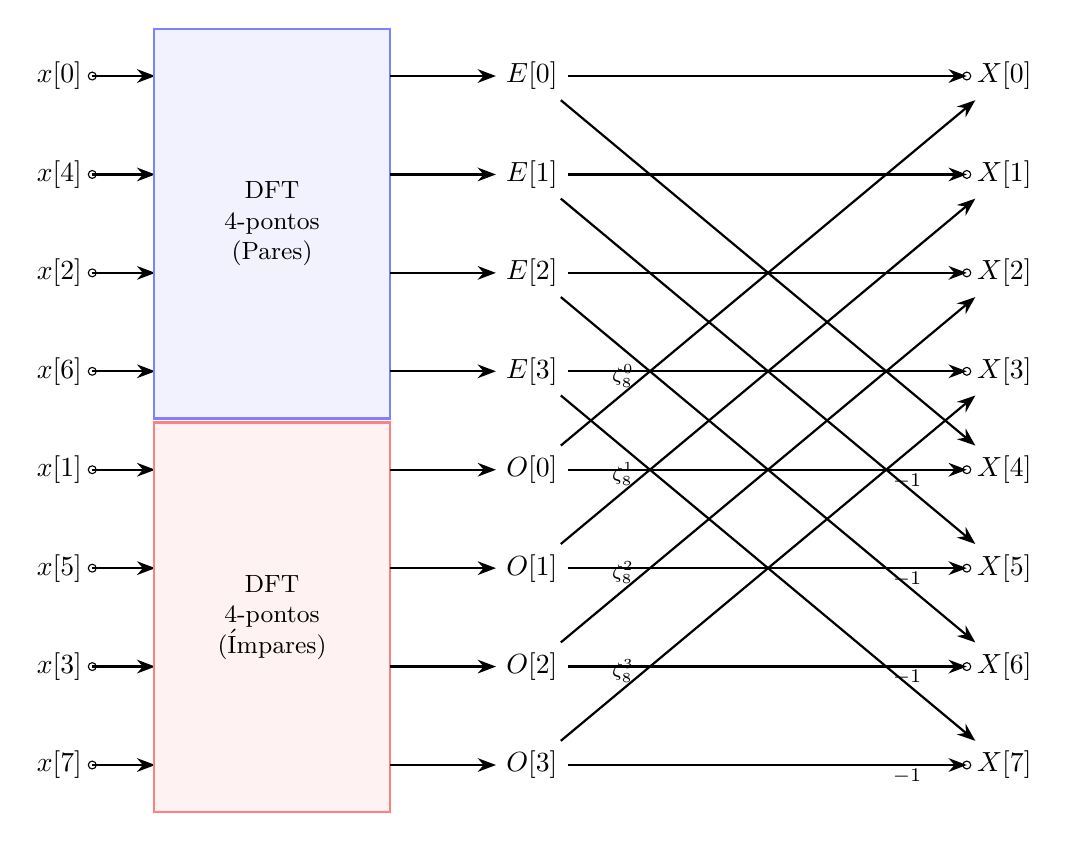
\begin{tikzpicture}[>=Stealth, node distance=1.5cm, thick]

  % --- CONFIGURAÇÕES GERAIS ---
  % Espaçamento vertical entre linhas
  \def\dy{1.25} % Reduzi ligeiramente para não ficar muito alto
  % Posições horizontais chaves
  \def\xBlockStart{1.2}
  \def\xBlockEnd{4.2}
  \def\xInter{6.0}
  \def\xFinal{12.0}
   
  % --- ENTRADA (Bit-Reversal N=8) ---
  % A ordem é: 0, 4, 2, 6 (Pares) | 1, 5, 3, 7 (Ímpares)
  
  % Grupo Pares (Evens)
  \node (x0) at (0, 0)      {$x[0]$};
  \node (x4) at (0, -\dy)   {$x[4]$};
  \node (x2) at (0, -2*\dy) {$x[2]$};
  \node (x6) at (0, -3*\dy) {$x[6]$};
  
  % Grupo Ímpares (Odds)
  \node (x1) at (0, -4*\dy) {$x[1]$};
  \node (x5) at (0, -5*\dy) {$x[5]$};
  \node (x3) at (0, -6*\dy) {$x[3]$};
  \node (x7) at (0, -7*\dy) {$x[7]$};

  % Pequenos círculos nos inputs e setas iniciais
  \foreach \n in {x0, x4, x2, x6, x1, x5, x3, x7} {
    \draw [fill=white, thin] (\n.east) circle (0.05);
    \draw [->] (\n.east) -- ++(0.8, 0);
  }

  % --- BLOCOS RECURSIVOS (N/2 DFTs) ---
  % Bloco Superior (DFT de 4 pontos para os Pares)
  % Abrange de y=0 até y=-3*dy
  \draw[fill=blue!5, draw=blue!50] (\xBlockStart, 0.6) rectangle (\xBlockEnd, -3*\dy - 0.6);
  \node at ({(\xBlockStart+\xBlockEnd)/2}, -1.5*\dy) [align=center, font=\small] {DFT\\4-pontos\\(Pares)};

  % Bloco Inferior (DFT de 4 pontos para os Ímpares)
  % Abrange de y=-4*dy até y=-7*dy
  \draw[fill=red!5, draw=red!50] (\xBlockStart, -4*\dy + 0.6) rectangle (\xBlockEnd, -7*\dy - 0.6);
  \node at ({(\xBlockStart+\xBlockEnd)/2}, -5.5*\dy) [align=center, font=\small] {DFT\\4-pontos\\(Ímpares)};

  % --- SAÍDAS INTERMEDIÁRIAS (E e O) ---
  % Saídas Pares (E0 a E3)
  \foreach \i in {0, 1, 2, 3} {
    \node (E\i) at (\xInter, -\i*\dy) {$E[\i]$};
  }
   
  % Saídas Ímpares (O0 a O3)
  \foreach \i in {0, 1, 2, 3} {
    % Calcula o deslocamento vertical correto (i + 4)
    \pgfmathtruncatemacro{\yidx}{\i+4}
    \node (O\i) at (\xInter, -\yidx*\dy) {$O[\i]$};
  }

  % Conectando blocos aos nós intermediários
  \foreach \i in {0, 1, 2, 3} {
     \draw [->] (\xBlockEnd, -\i*\dy) -- (E\i);
     \pgfmathtruncatemacro{\yidx}{\i+4}
     \draw [->] (\xBlockEnd, -\yidx*\dy) -- (O\i);
  }

  % --- ESTÁGIO DE COMBINAÇÃO FINAL (BUTTERFLY N=8) ---
   
  % Nós de Saída Final (X0 a X7)
  \foreach \i in {0,...,7} {
    \node (X\i) at (\xFinal, -\i*\dy) {$X[\i]$};
    % Círculos nas saídas
    \draw [fill=white, thin] (X\i.west) circle (0.05);
  }

  % --- CONEXÕES DO DIAGRAMA BORBOLETA ---
  % O loop principal percorre k = 0 a 3
  \foreach \k in {0, 1, 2, 3} {
    % Índice da segunda metade (k + N/2)
    \pgfmathtruncatemacro{\kplusfour}{\k+4}

    % --- Caminhos vindos de E[k] ---
    % E[k] contribui positivamente para X[k] e X[k+4]
    % Direto para X[k]
    \draw [->] (E\k) -- (X\k); 
    % Cruzado descendo para X[k+4]
    \draw [->] (E\k) -- (X\kplusfour); 

    % --- Caminhos vindos de O[k] ---
    % O[k] é multiplicado por W_8^k para X[k], e por -W_8^k para X[k+4]

    % Cruzado subindo para X[k] (Multiplicação pelo Twiddle Factor)
    % A posição pos=0.15 coloca o texto perto do início da linha (perto de O)
    \draw [->] (O\k) -- node[above, pos=0.15, font=\scriptsize, inner sep=2pt] {$\zeta_8^\k$} (X\k);
    
    % Direto para X[k+4] (Subtração / Multiplicação por -1)
    % A posição pos=0.85 coloca o texto perto do fim da linha (perto de X)
    \draw [->] (O\k) -- node[below, pos=0.85, font=\scriptsize, inner sep=1pt] {$-1$} (X\kplusfour);
  }

\end{tikzpicture}
\end{document}